\section{Problem 1: DIGITAL HALFTONING}\label{problem-1-digital-halftoning}
\textbf{sample1.png} is given in Figure 1.(a) Please apply several halftoning methods to the given image and provide discussions about the detail of the results.

Original image \nameref{sample1} for question \nameref{problem-1-digital-halftoning}.
\begin{figure}
    \centering
    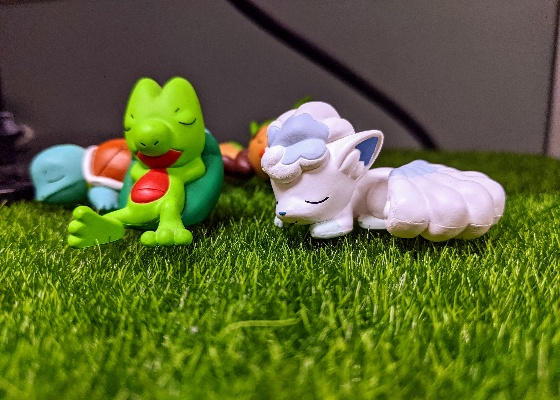
\includegraphics[scale=0.7]{src/sample1.png}
    \caption{\textbf{sample1.jpg}}
    \label{sample1}
\end{figure}

\subsection{(a)}\label{1_a}
Perform dithering using the dither matrix \(I_{2}\) in Figure 1.(b) and output the result as \textbf{result1.png}

\paragraph{Motivation}

\paragraph{Approach}

\paragraph{Performance of results}
In the end, I choose the \alert{settings}...

Result of problem 1(a): \nameref{result1}.
\begin{figure}
    \centering
    \includegraphics[scale=0.7]{src/result1.png}
    \caption{\textbf{result1.jpg} Dithering with \(I_{2}\)}
    \label{result1}
\end{figure}

\paragraph{Discussion}

\subsection{(b)}\label{1_b}
Expand the dither matrix \(I_{2}\) to \(I_{256}\) \((256 \times 256)\) and use it to perform dithering. Output the result as \textbf{result2.png}. Compare \textbf{result1.png} and \textbf{result2.png} along with some discussions.

\paragraph{Motivation}

\paragraph{Approach}

\paragraph{Performance of results}
In the end, I choose the \alert{settings}...

Result of problem 1(b): \nameref{result2}.
\begin{figure}
    \centering
    \includegraphics[scale=0.7]{src/result2.png}
    \caption{\textbf{result2.jpg} Dithering with \(I_{256}\)}
    \label{result2}
\end{figure}

\paragraph{Discussion}
Compare \textbf{result1.png} and \textbf{result2.png}...
\nameref{result2} sketch fine and smooth on the \textit{face of the cat}.

\subsection{(c)}\label{1_c}
Perform error diffusion with two different filter masks. Output the results as \textbf{result3.png}, and \textbf{result4.png}, respectively. Discuss these two masks based on the results. \\
You can find some masks \textbf{here} (from lecture slide 06. p23)

\paragraph{Motivation}

\paragraph{Approach}

\paragraph{Performance of results}
In the end, I choose the \alert{settings}...

Result of problem 1(c): \nameref{result3}.
\begin{figure}
    \centering
    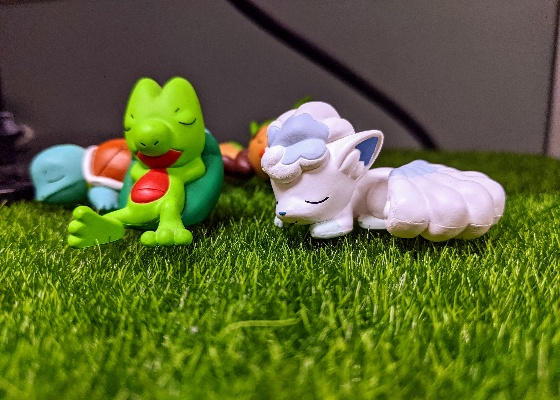
\includegraphics[scale=0.7]{src/sample1.png}
    \caption{\textbf{result3.jpg} Error diffusion with mask Floyd Steinberg}
    \label{result3}
\end{figure}

Result of problem 1(c): \nameref{result4}.
\begin{figure}
    \centering
    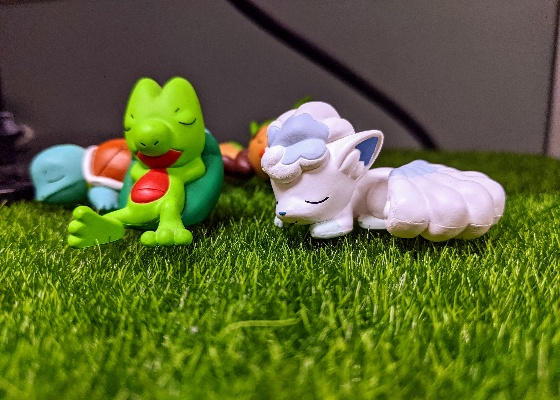
\includegraphics[scale=0.7]{src/sample1.png}
    \caption{\textbf{result4.jpg} Error diffusion with mask Jarvis}
    \label{result4}
\end{figure}

\paragraph{Discussion}
Discuss these two masks based on the results.

Other masks.

\subsection{(d)}\label{1_d}
Try to transfer \textbf{result1.png} to a dotted halftone/manga style binary image such as \textbf{sample1\_dotted.png} in Figure 1.(c). Describe the steps in detail and show the result. \\
You may need to utilize a function like \textbf{cv2.circle} to draw a circle.

\paragraph{Motivation}

\paragraph{Approach}

\paragraph{Performance of results}
In the end, I choose the \alert{settings}...

Result of problem 1(d): \nameref{result-prob1(d)}.
\begin{figure}
    \centering
    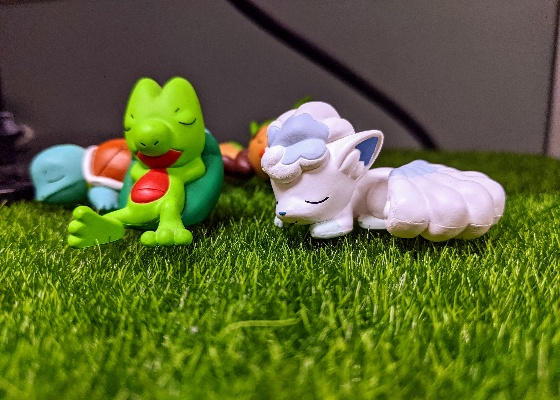
\includegraphics[scale=0.7]{src/sample1.png}
    \caption{\textbf{result-prob1(d).jpg} Dotted halftone style transfer}
    \label{result-prob1(d)}
\end{figure}

\paragraph{Discussion}
Interesting style transfer methods.
